\documentclass[class=minimal,border=0pt]{standalone}
\usepackage{tikz}
\usetikzlibrary{calc,arrows,shapes.multipart}

\begin{document}
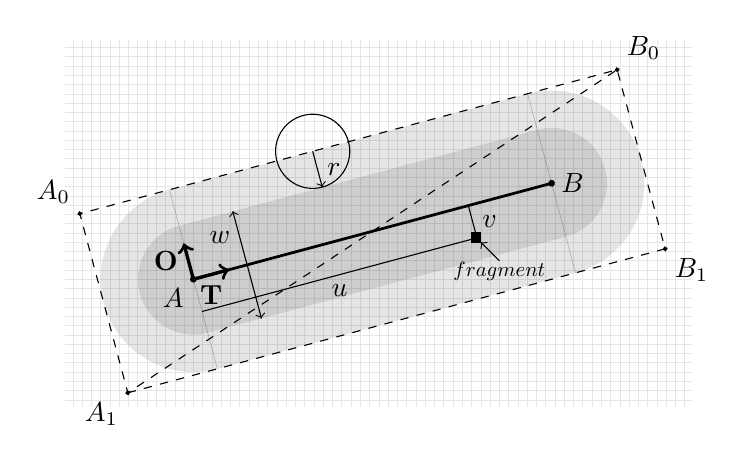
\begin{tikzpicture}[scale = .67]
  
  \begin{scope}[rotate = 15]
    \coordinate (A)  at (0pt,0pt);
    \coordinate (A0) at ($(A) + 50*(-1pt,+1pt)$);
    \coordinate (A1) at ($(A) + 50*(-1pt,-1pt)$);
    \coordinate (AO0) at ($(A) + 50*(0pt,+1pt)$);
    \coordinate (AO1) at ($(A) + 50*(0pt,-1pt)$);
    \coordinate (B)  at (200pt, 0pt);
    \coordinate (B0) at ($(B) + 50*(+1pt,+1pt)$);
    \coordinate (B1) at ($(B) + 50*(+1pt,-1pt)$);
    \coordinate (BO0) at ($(B) + 50*(0pt,+1pt)$);
    \coordinate (BO1) at ($(B) + 50*(0pt,-1pt)$);
    \coordinate (T)  at ($(A)!20pt!(B)$);
    \coordinate (O)  at ($(A)!20pt!90:(B)$);
    \coordinate (W0) at ($(A) + (+30pt,-30pt)$);
    \coordinate (W1) at ($(A) + (+30pt,+30pt)$);
    \coordinate (C0) at ($(A) + (+80pt,+50pt)$);
    \coordinate (C1) at ($(A) + (+80pt,+30pt)$);
    
    \draw[line width=67pt,cap=round,opacity=0.1] (A) -- (B);
    \draw[line width= 40pt,cap=round,opacity=0.1] (A) -- (B);
    \draw[line width=  1pt,cap=round] (A) -- (B);
    \draw[->,very thick] (A) -> (T) node[midway,below] {$\mathbf T$};
    \draw[->,very thick] (A) -> (O) node[midway,left]  {$\mathbf O$};
    \draw[<->] (W0) -- (W1) node[near end,left] {$w$};
    
    \filldraw [black] (A)  circle (1.5pt) node[anchor=north east] {$A$};
    \filldraw [black] (A0) circle (1pt) node[anchor=south east] {$A_0$};
    \filldraw [black] (A1) circle (1pt) node[anchor=north east] {$A_1$};
    \filldraw [black] (B)  circle (1.5pt) node[anchor=west]       {$B$};
    \filldraw [black] (B0) circle (1pt) node[anchor=south west] {$B_0$};
    \filldraw [black] (B1) circle (1pt) node[anchor=north west] {$B_1$};
    
    \draw[style=dashed] (A1) -- (B1) -- (B0) -- (A0) -- (A1) -- (B0);
    
    \draw[very thin, opacity=.25] (AO0) -- (AO1);
    \draw[very thin, opacity=.25] (BO0) -- (BO1);
    
    \draw [black] (C0) circle (20pt);
    \draw[->] (C0) -> (C1) node[midway,right] {$r$};
    
    \draw (0pt,-18pt) -- (153.5pt,-18pt) node[midway,below] {$u$};
    \draw (153.5pt,-18pt) -- (153.5pt,0pt) node[midway,right] {$v$};
  \end{scope}
  \draw[step=5pt,very thin,opacity=.1] (-69pt,-69pt) grid (269pt,129pt);
  \filldraw[] (150pt,20pt) rectangle (155pt,25pt);

  \filldraw[->] (165pt,10pt) node[below=-2pt,scale=.75] {$fragment$} -- (155pt,20pt);

\end{tikzpicture}
\end{document}
